\begin{figure}

\begin{minipage}{\linewidth}
\centering
\begin{minipage}{0.4\linewidth}
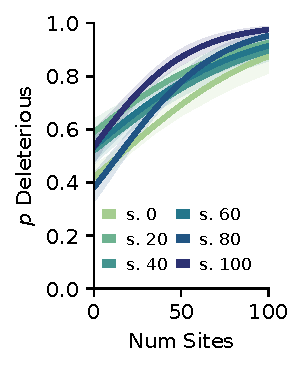
\includegraphics[width=\linewidth]{binder-2025-09-05-interpolation_complexity/binder/teeplots/2025-09-05-interpolation_complexity/bucket=prq49+endeavor=16+viz=plot-logistic-fit+ext=.pdf}
\end{minipage}%
\begin{minipage}{0.6\linewidth}
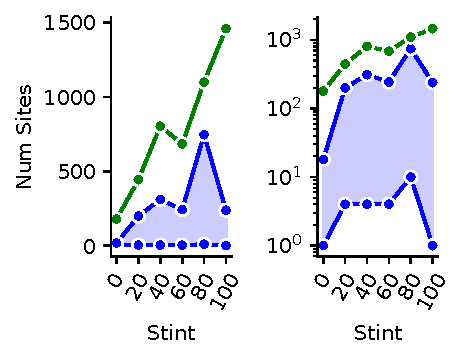
\includegraphics[width=\linewidth]{binder-2025-09-05-interpolation_complexity/binder/teeplots/2025-09-05-interpolation_complexity/bucket=prq49+endeavor=16+viz=plot-skeleton+ext=.pdf}
\end{minipage}
\end{minipage}

\vspace{-1ex}\textsc{}

\begin{minipage}{\linewidth}
\centering
\begin{subfigure}[t]{0.05\linewidth}
~
\end{subfigure}%
\begin{subfigure}[t]{0.4\linewidth}
\centering
\caption{\footnotesize knockout dose response}
\label{fig:cryptic:logistic}
\end{subfigure}%
\begin{subfigure}[t]{0.05\linewidth}
~
\end{subfigure}%
\begin{subfigure}[t]{0.5\linewidth}
\centering
\caption{\footnotesize skeleton size bounds}
\label{fig:cryptic:skeleton}
\end{subfigure}
\end{minipage}

\caption{
\textbf{Cryptic genome complexity.}
\footnotesize
Multi-site knockout assessments of genome content deemed neutral under single-site genome complexity screen.
Panel \ref{fig:cryptic:logistic} shows knockout dose responses, ranging up to 100-site knockouts.
Curves are logistic regressions, colored by specimen stint with shaded bootstrap 95\% CI.
Panel \ref{fig:cryptic:skeleton} reports ``skeleton'' size estimates --- a minimal set of non-critical sites necessary to maintain specimen fitness.
Upper skeleton bound is content under largest-sampled neutral knockout.
Lower skeleton size is a conservative estimate, based on probability of a complete skeleton set appearing in no larger knockout doses beyond last neutral knockout.
Log-scale plot included to show lower bound estimate.
Supplementary Figures \cref{fig:cryptic-interpolation-stint-0,fig:cryptic-interpolation-stint-20,fig:cryptic-interpolation-stint-40,fig:cryptic-interpolation-stint-60,fig:cryptic-interpolation-stint-80,fig:cryptic-interpolation-stint-100,} details underlying interpolation knockouts conducted at stints 0, 20, 40, 60, 80, and 100.
}
\label{fig:cryptic}

\end{figure}
